\chapter{Dagens pasientsignalsystem ved St. Olavs Hospital}
\label{appendix_dagenssystem}

St. Olavs Hospital er et universitetssykehus eid av Helse Midt-Norge RHF. I 2012 hadde sykehuset 131 547 inneliggende pasienter, 1 008 senger og 9 584 ansatte totalt. 
I dette appendikset vil vi beskrive dagens pasientsignalsystem, basert på informasjon gitt av Brukermanual for Pasientsignal og Pasientsignalapplikasjon (ref kilde).

\section{Pasientsignal}
Et pasientsignal utløses i et rom ved et sengetun for å tilkalle/alarmere pleiepersonell. Pasientsignalanlegget består av ulike trekkontaker og trykknapper, som pasientpanel \ref{pasientpanel}, rompanel \ref{rompanel} og vaktromsapparat \ref{vaktromsapparat}.

\begin{figure}
        \centering
        \begin{subfigure}[b]{0.3\textwidth}
                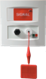
\includegraphics[scale=2]{pasientpanel.png}
                \caption{Pasientpanel}
                \label{pasientpanel}
        \end{subfigure}%
        \begin{subfigure}[b]{0.3\textwidth}
                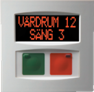
\includegraphics[scale=2]{rompanel.png}
                \caption{Rompanel}
                \label{rompanel}
        \end{subfigure}
        \begin{subfigure}[b]{0.3\textwidth}
                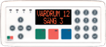
\includegraphics[scale=2]{vaktromsapparat.png}
                \caption{Vaktromsapparat}
                \label{vaktromsapparat}
        \end{subfigure}
        \caption{Pasientsignalanlegget}\label{pasientsignalanlegget}
\end{figure}

Disse er igjen tilkoblet andre IKT-komponenter:
Pasientsignalapplikasjon
Telefoni
Pasienterminal